\documentclass[11pt]{article}
\usepackage{pgfplots}
\pgfplotsset{compat=1.18}
\usepackage[utf8]{inputenc}
\usepackage[margin=1in]{geometry}
\usepackage{amsmath}
\usepackage{amssymb}
\usepackage{tabularx}
\usepackage{enumitem}
\usepackage{graphicx}
\usepackage{float}
\usepackage{titlesec}
\usepackage{pgfplotstable}
\usepackage{soul}
\usepackage{xcolor} 
\usepackage{booktabs}

\usepackage{siunitx} 
\usepackage{calligra}
\usepackage{enumitem}
\usepackage{changepage}
\usepackage[T1]{fontenc}
\usepackage{hyperref}
\usepackage{url}        
\usepackage[nottoc]{tocbibind}
\usepackage{caption}
\usepackage{array}
\usepackage{cancel}
\usepackage{chngcntr}
\usepackage{makecell}
\usepackage[authoryear,round]{natbib}
\usepackage{standalone} 
\usepackage{tikz}
\usepackage{newtxtext}
\usepackage{newtxmath}
\usepackage[dvipsnames]{xcolor}
\usetikzlibrary{calc, arrows.meta, angles, quotes}
\usetikzlibrary{decorations.pathmorphing}
\usetikzlibrary{arrows.meta,bending,shapes.geometric}
\DeclareCaptionFormat{justifiedbold}{
  \bfseries#1#2\normalfont#3
}
\captionsetup[figure]{format=justifiedbold, justification=justified, singlelinecheck=false, position=top}
\captionsetup[table]{format=justifiedbold, justification=justified, singlelinecheck=false, position=top}

\newenvironment{figtable}[1][h!]{
  \begin{figure}[#1]
  \centering
  \begin{tabular}{c}
}{
  \end{tabular}Experiment with different threshold
  \end{figure}
}

\newcommand{\vol}{\text{\reflectbox{\rotatebox[origin=c]{180}{A}}}}
\renewcommand{\thesection}{\Roman{section}.}
\renewcommand{\thesubsection}{\thesection\alph{subsection}}
\renewcommand{\thetable}{\thesubsection\arabic{table}}
\counterwithin{table}{subsection}

\newcommand{\greencheck}{^{\textcolor{green!70!black}{\checkmark}}}
\newcommand{\redcancel}[1]{{\color{red}\cancel{\color{black}#1}}}

\title{Simulink Model Of AUUV}
\author{Oscar Ivy}
\date{\today}

\begin{document}

\maketitle
\tableofcontents
\section{Introduction}
The purpose of this work is to develop a "Digital 
\section{Quadrotor Dynamics}


%Introduction to quadrotor Dynamics
{\tiny
"The quadrotor vehicle operates on the concept of variable torques and thrusts. Each rotor consists of a brushless DC motor and rotor with a fixed pitch. The motors are arranged in pairs along the horizontal and vertical axes with the forward pair rotating clockwise and the horizontal pair rotating counter-clockwise. This design results in the reaction torques from the pairs of motors being exactly opposed by each other if they are all spinning at the same speed. The elimination of the rotating moment allows the vehicle to maintain a constant heading while hovering. Yaw is controlled by varying the speeds of the pairs of motors to create a non-zero net counter torque. Altitude is controlled by varying the thrust from each motor by equal amounts to provide a net thrust vector and without a rotational moment. To move in the lateral directions, the relative speeds of each motor in the lateral pair are varied to create a desired lateral thrust offset. The simple design results in small platforms which are battery operated, able to perform a stable hover, and safe to use in indoor environments. The quadrotor is classified as an under-actuated system. While the quadrotor can move in 6 degrees of freedom (3 translational and 3 rotational), there are only 4 inputs that can be controlled (the speeds of the 4 motors). As will be shown below, the rotational and translational dynamics are coupled which presents an interesting control problem" -Wilselby (rephrase for our design) }

%Total List of assumptions made 
\subsection{Assumptions}
From Wilselby:
\begin{itemize}
    \item The quadrotor structure is rigid and symmetrical with a center of mass aligned with the center of the body frame of the vehicle.
    \item The thrust and drag of each motor is proportional to the square of the motor velocity.
    \item The propellers are considered to be rigid and therefore blade flapping is negligible (deformation of propeller blades due to high velocities and flexible material).
    \item The Earth is flat and non-rotating (difference of gravity by altitude or the spin of the earth is negligible)
    \item Surrounding fluid velocities (wind) are negligible.
    \item Ground effect is negligible.
\end{itemize}

%Relating Coordinate Frames
\subsection{Coordinate Frames}
{When designing a kinematic model of a system, one of the first considerations that must be made is the coordinate systems of interest. Every vector will act within one of these frames and with respect to them. The system we're designing for will receive positional information from IMUs (Internal Motion Unit). These units produce readings of acceleration and gyration with respect to axes that are attached to the body of the quadrotor. Additionally, an inertial frame is necessary so that the forces acting on the body can be converted into actual flight dynamics, with states that are in reference to a physical location in a "task space". } 
\subsubsection{Defining Coordinate Frames}
The first step I will take is to draw a simple diagram of the quadrotor in the task space, drawing on it two relevant frames, this can be seen in Figure [\ref{fig:GBF}].
\begin{figure}[H]
    \centering
    \caption{Relevant Frames and Parameters}
    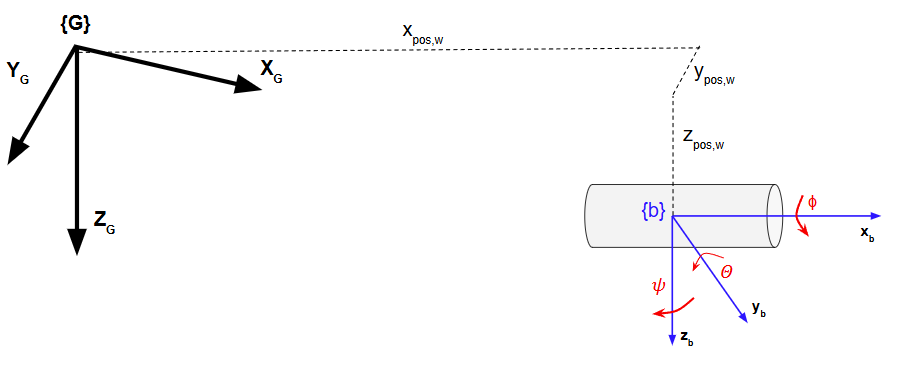
\includegraphics[width=0.8\linewidth]{GBF.png}
    \label{fig:GBF}
\end{figure}
\begin{itemize}
    \item body frame \{b\} ($x_b,y_b,z_b$): This frame is attached to the drone, it rotates and translates along with the $\text{rigid}^*$ body of the quadrotor. This frame is the frame in which all sensor measurements will be made.
    \item Global Frame \{G\} ($X^G,Y^G,Z^G$): this frame is the $\text{inertial}^*$ frame which allows for use of Newtons 2nd Law. Choosing North East and Down to be the X,Y, and Z axis respectively as it is a pretty standard notation for drones and other aircraft. 
\end{itemize}
As you can see in Figure [\ref{fig:GBF}], the position of the vehicle can be measured with respect to the Global Frame using position vectors. How though should the orientation of the vehicle be related to that of the Global Frame? 

\subsubsection{Coordinate Frame Transformations}
We need to be able to transform vectors between these two frames, given that all of our control inputs and sensor information take place in the body frame. Generally there are two methods used to achieve this, Euler angles and Quaternions.
\begin{center}
\large
    \textbf{\ul{Euler Angles}}
\end{center}
 Euler angles describe the transformation frome one frame to another as a series of rotations about its axes. A typically used sequence in Aerospace and Robotics applications is the Z-Y-X (yaw, pitch, roll)(3,2,1) sequence.
When using this sequence to transform from the body frame\{b\} to the global frame\{G\}, we first rotate about the $z_b$ axis by angle $\psi$, and arrive at the first intermediate frame \{b'\} with axes ($x_b'\;,y_b'\,,z_b'$). Then, we rotate about $y_b'$ by angle $\theta$ (pitching the vehicle), arriving at the second intermediate frame  \{b''\} with axes ($x_b''\;,y_b''\,,z_b''$). Finally rotating about the $x'_b$ axis by angle $\phi$ (roll), and arrive at Frame \{G\}. These steps are visualized below, and are valid for any transformation between axis.
\begin{center}
    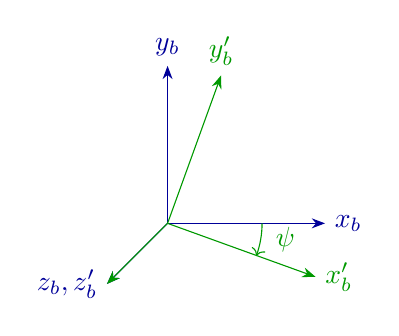
\begin{tikzpicture}
        \draw [blue!60!black][-Stealth](0,0,0) -- (0,0,2) node [left]{$z_b,z'_b$};
        \draw [blue!60!black][-Stealth](0,0,0) -- (0,2,0) node [above]{$y_b$};
        \draw [blue!60!black][-Stealth](0,0,0) -- (2,0,0) node [right]{$x_b$};

        \draw [green!60!black][-Stealth](0,0,0) -- (1.88,-0.68,0) node [right]{$x'_b$};
        \draw [green!60!black][-Stealth](0,0,0) -- (0.68,1.88,0) node [above]{$y'_b$};
        \draw [green!60!black][-Stealth](0,0,0) -- (0,0,2) ;
        \draw [green!60!black, ->] (1.2,0,0) arc (0:-20:1.2) node [midway, right=2pt] {$\psi$};
    \end{tikzpicture}
    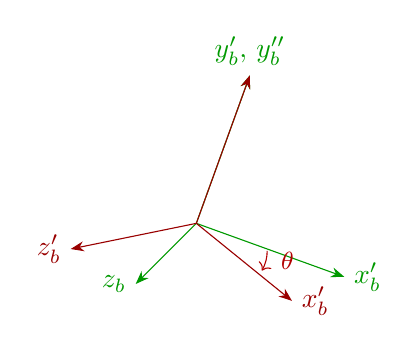
\begin{tikzpicture}
        \draw [green!60!black][-Stealth](0,0,0) -- (1.88,-0.68,0) node [right]{$x'_b$};
        \draw [green!60!black][-Stealth](0,0,0) -- (0.68,1.88,0) node [above]{$y'_b,\,y''_b$};
        \draw [green!60!black][-Stealth](0,0,0) -- (0,0,2) node [left]{$z_b$};
        
        \draw [red!60!black][-Stealth](0,0,0) -- (1.6,-0.6,1) node [right]{$x'_b$};
        \draw [red!60!black][-Stealth](0,0,0) -- (0.68,1.88,0) ;
        \draw [red!60!black][-Stealth](0,0,0) -- (-0.93,0.34,1.73)node [left]{$z'_b$} ;
        
        \draw [red!70!black, ->] (.9,-0.35,0) arc (0:-30:0.5) node [midway, right=2pt] {\small$\theta$};
    \end{tikzpicture}
    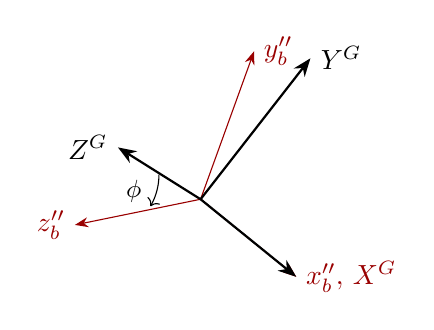
\begin{tikzpicture}
        \draw [red!60!black][-Stealth](0,0,0) -- (1.6,-0.6,1) node [right]{$x''_b,\,X^G$};
        \draw [red!60!black][-Stealth](0,0,0) -- (0.68,1.88,0) node [right]{$y''_b$};
        \draw [red!60!black][-Stealth](0,0,0) -- (-0.93,0.34,1.73)node [left]{$z''_b$} ;
        
        \draw [black,thick][-Stealth](0,0,0) -- (1.6,-0.6,1) ;
        \draw [black,thick][-Stealth](0,0,0) -- (1.062,1.457,-0.866) node [right]{$Y^G$};
        \draw [black,thick][-Stealth](0,0,0) -- (-0.472,1.236,1.5)node [left]{$Z^G$} ;
        
        \draw [ ->] (-0.24,0.6,0.75) arc (0:-30:0.8) node [midway, left=2pt] {\small$\phi$};
    \end{tikzpicture}
\end{center}
These rotations can be described with trigonometric functions, for example, from frame $b \xrightarrow{} b'$:
\begin{align*}
    x'_b &=\cos(\psi)x_b-sin(\psi)y_b\\
    y'_b &=  \sin(\psi)x_b +\cos(\psi)\,y_b \\
    z'_b &= z_b
\end{align*}
In  Matrix Form this becomes:
$$\begin{bmatrix}
    x'_b\\y'_b\\z'_b
\end{bmatrix} = 
\begin{bmatrix}
    \cos(\psi) & -\sin(\psi) & 0\\
    \sin(\psi) & \cos(psi) & 0\\
    0 & 0& 1
\end{bmatrix}\begin{bmatrix}
    x_b\\y_b\\z_b
\end{bmatrix}$$
Repeating this process for rotations about each successive axis we get the following matrices:

$$
    R_x(\phi) = \begin{bmatrix}
        1&0&0\\0&\cos\phi&-\sin\phi&\\0&\sin\phi&cos\phi
    \end{bmatrix},\;\;
    R_y(\theta) =\begin{bmatrix}
        \cos\theta&0&\sin\theta\\0&1&0\\-\sin\theta&0&\cos\theta
    \end{bmatrix},\;\;
    R_z(\psi) = \begin{bmatrix}
        \cos\psi & -\sin\psi &0\\\sin\psi&\cos\psi & 0\\0&0&1
    \end{bmatrix}
$$
Post multiplying the Standard Z-Y-X Euler Sequence to get the final rotational matrix from the body frame to the global frame$R_b^G$:
$$R_b^G = R_z(\psi) R_y(\theta) R_x(\phi) = \begin{bmatrix} \cos\psi & -\sin\psi & 0 \\ \sin\psi & \cos\psi & 0 \\ 0 & 0 & 1 \end{bmatrix} \begin{bmatrix} \cos\theta & 0 & \sin\theta \\ 0 & 1 & 0 \\ -\sin\theta & 0 & \cos\theta \end{bmatrix} \begin{bmatrix} 1 & 0 & 0 \\ 0 & \cos\phi & -\sin\phi \\ 0 & \sin\phi & \cos\phi \end{bmatrix}$$
\begin{equation} R_b^G = \begin{bmatrix}   c_\psi c_\theta &  c_\psi s_\theta s_\phi -  s_\psi c_\phi &  c_\psi s_\theta c_\phi +  s_\psi s_\phi \\  s_\psi c_\theta &  s_\psi s_\theta s_\phi +  c_\psi c_\phi &  s_\psi s_\theta c_\phi -  c_\psi s_\phi \\ - s_\theta &  c_\theta s_\phi &  c_\theta c_\phi  
\end{bmatrix}
\label{eq:R_b^G}\end{equation}




\subsubsection{Kinematic Relationship Between Body Rates and Euler Rates}
Given that the euler angles (and therefore rates) occur in a ZYX sequence as shown in the previous section, and, the body rates occur in the final transformed frame, the two must be related via a series of rotations. Following the ZYX rotation our euler angles measure the following:

\begin{itemize}
    \item Yaw ($\psi$): Rotation about the initial inertial $Z$-axis ($Z_0$) by angle $\psi$.
    \item Pitch ($\theta$): Rotation about the intermediate $y'$-axis by angle $\theta$.
    \item Roll ($\phi$): Rotation about the final body $x''$-axis (or $x_b$) by angle $\phi$.
\end{itemize}
Meaning, the angular velocity of each would be defined:

\begin{itemize}
    \item $\dot{\psi}$ acts along the inertial $Z_0$-axis: $\boldsymbol{\omega}_{\psi} = [0, 0, \dot{\psi}]^T$
    \item $\dot{\theta}$ acts along the intermediate $y'$-axis: $\boldsymbol{\omega}_{\theta} = [0, \dot{\theta}, 0]^T$
    \item $\dot{\phi}$ acts along the body $x_b$-axis: $\boldsymbol{\omega}_{\phi} = [\dot{\phi}, 0, 0]^T$
\end{itemize}
\textbf{Transforming Rates to the Body Axis:}\\
\noindent The first derivative of \textit{roll} ($\dot{\phi}$) already acts along the body $x_b$-axis, and therefore can be simply defined:
$$\boldsymbol{\omega}_{\phi}^B = \begin{bmatrix} \dot{\phi} \\ 0 \\ 0 \end{bmatrix}$$

\noindent The first derivative of \textit{pitch} ($\dot{\theta}$) acts along the intermediate y' axis, and, therefore must be rotated by $\phi$ about the x-axis: 
$$\boldsymbol{\omega}_{\theta}^B = R_x(\phi) \begin{bmatrix} 0 \\ \dot{\theta} \\ 0 \end{bmatrix} = \begin{bmatrix} 1 & 0 & 0 \\ 0 & \cos\phi & -\sin\phi \\ 0 & \sin\phi & \cos\phi \end{bmatrix} \begin{bmatrix} 0 \\ \dot{\theta} \\ 0 \end{bmatrix}$$
 $$\boldsymbol{\omega}_{\theta}^B= \begin{bmatrix} 0 \\ \dot{\theta}\cos\phi \\ \dot{\theta}\sin\phi \end{bmatrix}$$
\noindent The first derivative of \textit{yaw} ($\dot{\psi}$) acts along the inertial $Z_o$-axis and therefore must be rotated twice (by the pitch angle and roll angle). 
$$\boldsymbol{\omega}_{\psi}^B = R_x(\phi) R_y(\theta) \begin{bmatrix} 0 \\ 0 \\ \dot{\psi} \end{bmatrix} = \begin{bmatrix} 1 & 0 & 0 \\ 0 & \cos\phi & -\sin\phi \\ 0 & \sin\phi & \cos\phi \end{bmatrix} \begin{bmatrix} \cos\theta & 0 & \sin\theta \\ 0 & 1 & 0 \\ -\sin\theta & 0 & \cos\theta \end{bmatrix} \begin{bmatrix} 0 \\ 0 \\ \dot{\psi} \end{bmatrix}$$
$$\boldsymbol{\omega}_{\psi}^B = \begin{bmatrix} -\dot{\psi}\sin\theta \\ \dot{\psi}\cos\theta\sin\phi \\ \dot{\psi}\cos\theta\cos\phi \end{bmatrix}$$
\textbf{Summing components to form $\omega^B$}
$$\begin{bmatrix} p \\ q \\ r \end{bmatrix} = \boldsymbol{\omega}_{\phi}^B + \boldsymbol{\omega}_{\theta}^B + \boldsymbol{\omega}_{\psi}^B = \begin{bmatrix} \dot{\phi} - \dot{\psi}\sin\theta \\ \dot{\theta}\cos\phi + \dot{\psi}\cos\theta\sin\phi \\ -\dot{\theta}\sin\phi + \dot{\psi}\cos\theta\cos\phi \end{bmatrix}$$
Re-writing this expression in Matrix form, we get a matrix that maps Euler rates to body rates:
$$\begin{bmatrix} p \\ q \\ r \end{bmatrix} = \begin{bmatrix} 1 & 0 & -\sin\theta \\ 0 & \cos\phi & \cos\theta\sin\phi \\ 0 & -\sin\phi & \cos\theta\cos\phi \end{bmatrix} \begin{bmatrix} \dot{\phi} \\ \dot{\theta} \\ \dot{\psi} \end{bmatrix}$$
Inverting the matrix gives a matrix which maps body rates to euler rates: 
\begin{equation}\begin{bmatrix} \dot{\phi} \\ \dot{\theta} \\ \dot{\psi} \end{bmatrix} = \begin{bmatrix} 1 & \sin\phi\tan\theta & \cos\phi\tan\theta \\ 0 & \cos\phi & -\sin\phi \\ 0 & \frac{\sin\phi}{\cos\theta} & \frac{\cos\phi}{\cos\theta} \end{bmatrix}\begin{bmatrix} p \\ q \\ r \end{bmatrix}\end{equation}

\noindent If the Euler Angles of the quadrotor are assumed to be small during flight ($\le 10^o)$, the small angle assumption can be used which will turn the matrix above into the \textit{identity matrix} such that the body rates are roughtly equal to the first derivative of the euler angles. \vspace{0.5cm}
\\
\hl{\textbf{A note on Gimbal Lock}}\\
Given the physical limitations of our robot and its specific use case, we never intend to command our drone to any large pitch angles. However, in equation (2) you can see clearly where gimbal lock could become an issue in this approach. Should $\theta$ approach $90^o$, the two terms in the third row with $\theta$ in the denominator would approach infinity and the kinematics would break. This is called gimbal lock and it represents a possible singularity. For this reason, quaternions are often used for kinematics of a quadrotor. However, as stated, this shouldn't be an issue in our use case.  

\section{Forces and Moments in the Body Frame}
For now, we'll focus on aerial flight with no wind, leaving us with really three forces of concern. 
\begin{enumerate}
    \item Thrust force felt from combination of rotor thrusts
    \item Drag on the vehicle
    \item Effects of Gravity (weight)
\end{enumerate}
\subsection{Rotor Thrust}
\subsubsection{Power Draw}
Before jumping into the mixing of the motor thrusts, we will first consider a first principal approach to the motor power we can expect to be drawn. Starting with the information we're given about motor specs RPM per V or KV:
$$KV^* = \frac{RPM}{V}$$
Converting to SI Units:
$$\frac{rad/s}{V} = \frac{\text{rot/min}}{V}\frac{(2\pi \text{ rad})/(60 s)}{1}= \frac{KV^*\cdot2\pi}{60}$$
The inverse of this ratio is the theoretical back emf constant ($K_v$), or, the voltage created in the brush-less motors by their motion.  $$K_v = \frac{V}{rad/s} = \frac{60}{KV^*\cdot2\pi} $$ 
Another parameter of interest is the Torque per Amp ($K_t = \frac{Nm}{A}$). It can be shown that This parameter is equivalent to the theoretical back emf ($K_t = K_v$). Starting with the expression for electrical and rotational power:
$$P_e = IV\;\;\;P_r = \tau\omega$$
Where I = current, V = voltage, $\tau$ = torque, and $\omega$=angular velocity. Here, only examining the electric power consumed by the motors ($P_e = P_m$). 
\begin{align*}
IV &= \tau\omega
\intertext{Rearranging: }
\frac{\tau}{I} &=\frac{V}{\omega}
\intertext{In Si Units:}
\frac{N\cdot m}{A} &= \frac{V}{\text{rad/s}}
\intertext{This gives us:}
&\boxed{K_t = K_v =\frac{60}{KV^*\cdot2\pi} }
\end{align*}
\\
\noindent We can express the torque as a function of ($K_t$):
$$\tau = K_t(I-I_o)$$ Where $I_o$ is the "No-load current", another motor spec which it typically given with a motor. This is the current at which the motor operates and generates 0 torque. Increases in current after this will scale with $K_t$. Solving for current we get the expression:
$$I =\frac{\tau}{K_t}+I_o $$
Here we will model the Voltage to be the standard $V=IR$ plus the back emf created by the motors governed by the theoretical back emf coefficient ($K_v$) dervied earlier:
$$V = IR_m + K_v\omega$$
Where $R_m$ is the motor resistance, this is a value in ohms and is also typically included in a motors spec sheet. We can substitute these values for voltage and current into the equation for electric power:
\begin{align*}
    P_e&=IV=\left(\frac{\tau}{K_t}+I_o \right)\left( IR_m + K_v\omega\right)
    \intertext{substituting I into the expression for V:}
    P_e&=\left(\frac{\tau}{K_t}+I_o \right)\left[ \left(\frac{\tau}{K_t}+I_o\right)R_m + K_v\omega\right]
    \intertext{substituting in the expression for $K_t=K_v$:}
    P_e&=\left(\frac{\tau}{\frac{60}{KV^*\cdot2\pi}}+I_o \right)\left[ \left(\frac{\tau}{\frac{60}{KV^*\cdot2\pi}}+I_o\right)R_m + \frac{60}{KV^*\cdot2\pi}\omega\right]\\
    P_e&=\left(\frac{\tau KV^*\cdot2\pi}{60}+I_o \right)\left[ \left(\frac{\tau KV^*\cdot2\pi}{60}+I_o\right)R_m + \frac{60}{KV^*\cdot2\pi}\omega\right]
\end{align*}
Torque Generated by propellors on a motor is governed by their drag coefficient ($k_m$) this coefficient is sometimes included along with a propellors data sheet although it can also be determined through experimentation using a test stand which monitors the torque generated, and fits it to a line of the form:
$$\tau = k_m\omega^2$$
Substituting this equation into our expression for electric power consumption:
$$
    P_e=\left(\frac{ k_m\omega^2 KV^*\cdot2\pi}{60}+I_o \right)\left[ \left(\frac{ k_m\omega^2 KV^*\cdot2\pi}{60}+I_o\right)R_m + \frac{60}{KV^*\cdot2\pi}\omega\right]$$
$$
    P_e= \left(\frac{ k_m\omega^2 KV^*\cdot2\pi}{60}+I_o\right)^2R_m + \frac{60\;\omega}{KV^*\cdot2\pi}\left(\frac{ k_m\omega^2 KV^*\cdot2\pi}{60}+I_o \right)$$
$$\boxed{
    P_e= R_m\left(\frac{ k_m\omega^2 KV^*\cdot2\pi}{60}+I_o\right)^2 + k_m\omega^3+\frac{60I_o\omega}{2\pi(KV^*)}}$$

This makes $P_e= f(\omega)$ and constants. By designing for a $\omega_{req}$, we can determine the power draw from the motors and, therefore, flight times. The thrust required for hover is:
\begin{align*}
T_{\text{total}} &= mg \\
\intertext{With four motors each producing $f_{\text{thrust}}$:}
4f_{\text{thrust}} &= mg \\
\intertext{Using the aerodynamic thrust relationship $f_{\text{thrust}} = k_f \omega^2$:}
4 k_f \omega_{\text{hover}}^2 &= mg
\intertext{Solving for $\omega_{hover}$}
\omega_{hover} &= \sqrt{\frac{mg}{4k_f}}\;\;\;(rad/s)
\end{align*}
Plugging this into our expression for $P_e$ gives us a realistic estimate of the power draw due to the motors: 
$$\boxed{
    P_e= R_m\left(\frac{ k_mmg KV^*2\pi}{604k_f}+I_o\right)^2 + k_m\sqrt{\frac{mg}{4k_f}}^3+\frac{60I_o\sqrt{\frac{mg}{4k_f}}}{2\pi(KV^*)}}$$
\subsubsection{Flight Time}
To finish this section regarding motor power, we will define a model for determining the runtime of the system as a function of it's mass (or g's of acceleration by scaling based on mass such that 1g = nominal mass, 2g = 2*(nominal mass)). Batteries have three constants of interest for these calculations: Capacity (Ah), Nominal Voltage (V), Efficiency. Using these constants and the electrical power draw from the motors determined in the previous section we get to this equation:
$$\text{Usable Runtime (hours)} = \frac{\text{Capacity(Ah)}\times\text{ Nominal Voltage(V)}}{\text{Power Draw (Watts)}} \times \text{Efficiency Factor}$$
\subsection{Translational Dynamics}
The equations of motion are defined in the 'inertial' global reference frame. Using Newtons 2nd Law, acceleration of the quadrotor in this frame is equal to the sum of forces multiplied by the mass of the quadrotor. The sum of forces is comprised of the force of gravity ($F_g$), thrust of the motors translated from the body frame to the global inertial frame ($F_T^G$), and and the drag force ($F_d$). 
\begin{figure}[H]
    \centering
    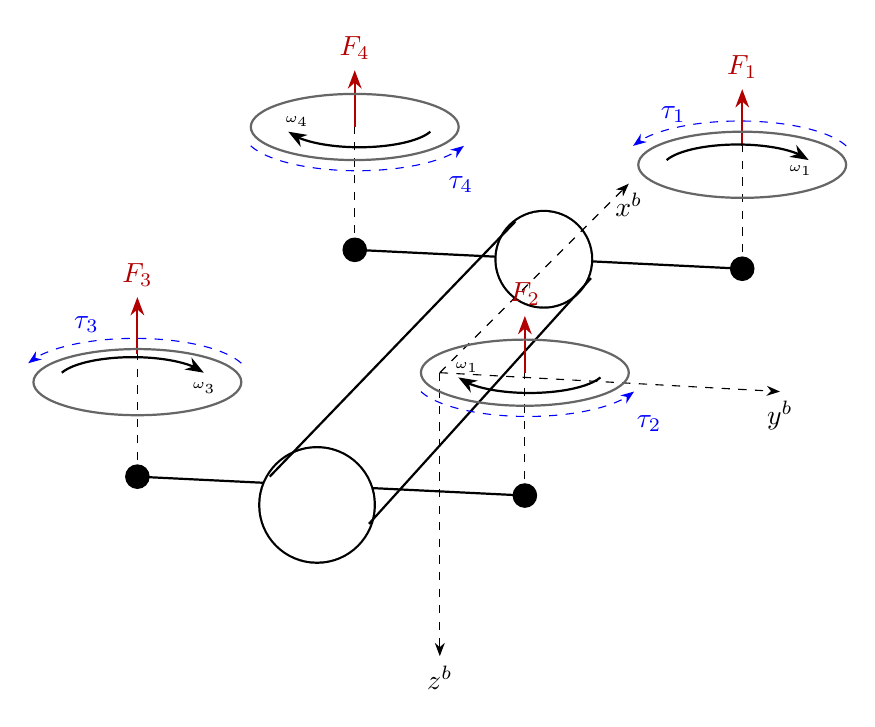
\begin{tikzpicture}[scale=1.2, >=Stealth, font=\sffamily]

  % Define key coordinates (3D projection)
  \coordinate (O) at (0, 0);          % Center origin
  \coordinate (M1) at (3.2, 1.1);     % Motor 1 (Front/Right)
  \coordinate (M2) at (0.9, -1.3);    % Motor 2 (Rear/Right)
  \coordinate (M3) at (-3.2, -1.1);   % Motor 3 (Rear/Left)
  \coordinate (M4) at (-0.9, 1.3);    % Motor 4 (Front/Left)
  

  % Draw Body Frame Axes
  % x^b axis (dashed extend past motor 1)
  \draw[thick] (M3) -- (M2);
  \draw[thick] (M1) -- (M4);
  \draw[ultra thick] (M1) ++(-4.5, -2.5) ellipse (0.6cm and 0.6cm);
  \draw[ultra thick] (M1) ++(-2.1, 0.1) ellipse (0.5cm and 0.5cm);
  \fill[white] (M1) ++(-4.5, -2.5) ellipse (0.6cm and 0.6cm);
  \fill[white] (M1) ++(-2.1, 0.1) ellipse (0.5cm and 0.5cm);
\draw [thick](-1.8,-1.1) --(0.8,1.6);
\draw [thick](-0.75,-1.6) --(1.6,1);
  % z^b axis (pointing downwards)
  \draw[dashed, ->] (O) -- (0, -3) node[below] {$z^b$};
  \draw[dashed, ->] (O) -- (2, 2) node[below] {$x^b$};
  \draw[dashed, ->] (O) -- (3.6, -0.2) node[below] {$y^b$};

  % Motor Hubs (Filled Rounded Rectangles/Nodes)
  \foreach \m in {M1, M2, M3, M4} {
    \node[draw, fill=black, circle, inner sep=3pt] at (\m) {};
  }

  % --- MOTOR 1 (Counter-Clockwise Rotation) ---
  \draw[dashed] (M1) -- ++(0, 1.3);
  \draw[thick, ->,red!70!black] (M1) ++(0, 1.3) -- ++(0, 0.6) node[above] {$F_1$};
  % Rotor Disk
  \draw[thick, gray!80!black] (M1) ++(0, 1.1) ellipse (1.1cm and 0.35cm);
  % Rotation arrow inside
  \draw[thick, ->] (M1) ++(-0.8, 1.15) arc (160:20:0.8cm and 0.25cm) node [below,pos=0.9] {\tiny $\omega_1$};
  % Torque arrow outside
  \draw[dashed, ->,blue] (M1) ++(1.1, 1.3) arc (20:160:1.2cm and 0.4cm) node[pos = 0.9, above right=2pt] {$\tau_1$};

  % --- MOTOR 2 (Clockwise Rotation) ---
  \draw[dashed] (M2) -- ++(0, 1.3);
  \draw[thick, ->,red!70!black] (M2) ++(0, 1.3) -- ++(0, 0.6) node[above] {$F_2$};
  % Rotor Disk
  \draw[thick, gray!80!black] (M2) ++(0, 1.3) ellipse (1.1cm and 0.35cm);
  % Rotation arrow inside
  \draw[thick, ->] (M2) ++(0.8, 1.25) arc (-20:-160:0.8cm and 0.25cm) node [pos=0.9, above] {\tiny $\omega_1$};
  % Torque arrow outside
  \draw[dashed, ->,blue] (M2) ++(-1.1, 1.1) arc (200:340:1.2cm and 0.4cm) node[pos = 0.9, below right=2pt] {$\tau_2$};

  % --- MOTOR 3 (Counter-Clockwise Rotation) ---
  \draw[dashed] (M3) -- ++(0, 1.3);
  \draw[thick, ->,red!70!black] (M3) ++(0, 1.3) -- ++(0, 0.6) node[above] {$F_3$};
  % Rotor Disk
  \draw[thick, gray!80!black] (M3) ++(0, 1) ellipse (1.1cm and 0.35cm);
  % Rotation arrow inside
  \draw[thick, ->] (M3) ++(-0.8, 1.1) arc (160:20:0.8cm and 0.25cm) node [pos=1, below] {\tiny$\omega_3$};
  % Torque arrow outside
  \draw[dashed, ->, blue] (M3) ++(1.1, 1.2) arc (20:160:1.2cm and 0.4cm) node[pos=0.8, above right=2pt] {$\tau_3$};

  % --- MOTOR 4 (Clockwise Rotation) ---
  \draw[dashed] (M4) -- ++(0, 1.3);
  \draw[thick, ->,red!70!black] (M4) ++(0, 1.3) -- ++(0, 0.6) node[above] {$F_4$};
  % Rotor Disk
  \draw[thick, gray!80!black] (M4) ++(0, 1.3) ellipse (1.1cm and 0.35cm);
  % Rotation arrow inside
  \draw[thick, ->] (M4) ++(0.8, 1.25) arc (-20:-160:0.8cm and 0.25cm) node [above,pos = 0.9] {\tiny$\omega_4$};
  % Torque arrow outside
  \draw[dashed, ->,blue] (M4) ++(-1.1, 1.1) arc (200:340:1.2cm and 0.4cm) node[pos=0.8, below right=2pt] {$\tau_4$};
\end{tikzpicture}
    \caption{Caption}
    \label{fig:TikzRotors}
\end{figure}


\noindent\ul{$\mathbf{\sum F = ma|}:$}



$$m\ddot{X}^G = F_g+F_d+F_T^G $$

Where $\ddot{X}^G$ is the second derivative of the X,Y,Z position vector in the global frame. \\

\noindent\textbf{ \ul{Force of Gravity In Global Frame|}:}\vspace{0.2cm}\\
In the global frame, gravity is always pointed down, this is aligned with the z axis in the NED convention, and therefore, the gravity vector in the global frame can be defined:
$$\boxed{F_g = \begin{bmatrix}
0\\0\\mg
\end{bmatrix}}$$

\noindent\textbf{ \ul{Drag Force|}:}\vspace{0.2cm}\\
\noindent Since the environment is assumed to have no wind (for now), the drag force modeled here is essentially a pure resistance to motion (a dampening term). Here, we will use a simplified model of drag that treats drag as proportionally linear to velocity in the global frame. The coefficients of drag, however, will be specific to the geometry of the quadrotor, and therefore, it's orientation. Because of this it is necessary to first translate the velocities in the global frame to the body frame. Using Equation [\ref{eq:R_b^G}] $R_b^G$, where it can be shown that $R_G^b = [R_b^b]^T$ (true for any true rotational matrix) and therefore: $$\begin{bmatrix} \dot{x}_b\\\dot{y}_b\\\dot{z}_b\end{bmatrix}=R_G^b\begin{bmatrix} \dot{X}^G\\\dot{Y}^G\\\dot{Z}^G\end{bmatrix} = [R_b^G]^T \begin{bmatrix}\dot{X}^G\\\dot{Y}^G\\\dot{Z}^G \end{bmatrix}$$ 

\noindent As mentioned, the drag force depends on geometries in the body frame, and, is modeled proportionally linear with respect to velocity. Using the expression above for velocity in the body frame, and $K_{d,x},\,K_{d,y},\,\text{and }K_{d,z}$ represent the coefficient of drag for the x,y, and z axis of the body frame:
$$F_d^b =\begin{bmatrix}
    K_{d,x}&0&0\\0&K_{d,y}&0\\0&0&K_{d,z}
\end{bmatrix}[R_b^G]^T \begin{bmatrix}\dot{X}^G\\\dot{Y}^G\\\dot{Z}^G \end{bmatrix} $$
\noindent Or:
$$F_d^b =K_d[R_b^G]^T \begin{bmatrix}\dot{X}^G\\\dot{Y}^G\\\dot{Z}^G \end{bmatrix} $$
\noindent Where $K_d$ is defined:
\begin{equation} K_d =\begin{bmatrix}
    K_{d,x}&0&0\\0&K_{d,y}&0\\0&0&K_{d,z}
\end{bmatrix}\label{eq:K_d}
\end{equation}\\
\\\noindent Converting these forces back into the global frame, for the final equation of the drag force vector in the global frame. 
\begin{equation*}
    \boxed{F_d^G =\,R_b^G\cdot K_d\cdot[R_b^G]^T \cdot \begin{bmatrix}\dot{X}^G\\\dot{Y}^G\\\dot{Z}^G \end{bmatrix}}
    \label{eq:F_d^G}
\end{equation*}

\noindent\textbf{ \ul{Thrust Force|}:}\vspace{0.22 cm}\\
In the Body frame, the thrust vector acts only in the $-z_b$ direction, as shown in Figure [\ref{fig:TikzRotors}] additionally, as discussed previously, for each (i) motor, the magnitude of the thrust generated is modeled as $F_i = K_T\cdot\omega_i^2$ where $K_T$ is the coefficient of thrust (constant for each motor). Therefore, the total thrust Force (T) can be defined as the sum of the individual thrusts of each motor. \begin{equation}
    T=\sum^4_{i=1}F_i = \sum^4_{i=1}K_{T,i}\,\cdot\omega_i^2 = K_{T_1}\omega^2_1+K_{T_2}\omega^2_2+K_{T_3}\omega^2_3+K_{T_4}\omega^2_4
    \label{eq:T}
\end{equation}
This gives us:
$$F_T^b  = -\begin{bmatrix}
    0\\0\\T
\end{bmatrix} =T\begin{bmatrix}
    0\\0\\1
\end{bmatrix}  $$
Using equation (\ref{eq:R_b^G}) for $R_b^G$ we can rotate the thrust force in the body frame into forces in the global frame:

\begin{equation*}
    \boxed{F_T^G =-T\,R_b^G\begin{bmatrix}
    0\\0\\1
\end{bmatrix}}
\label{eq:F_T^G}
\end{equation*} 


\noindent\textbf{\ul{Summing the Gravity, Drag, and Thrust forces|}:}
$$m\ddot{X}^G = F_g+F_d+F_T^G $$
$$m\ddot{X}^G = \begin{bmatrix}
0\\0\\mg
\end{bmatrix}-\,R_b^G\, K_d\,[R_b^G]^T \begin{bmatrix}\dot{X}^G\\\dot{Y}^G\\\dot{Z}^G \end{bmatrix}-TR_b^G\begin{bmatrix}
    0\\0\\1
\end{bmatrix} $$
\textbf{\ul{Dividing mass to determine acceleration in the body frame|}:}
\begin{equation}\boxed{\ddot{X}^G = \begin{bmatrix}
0\\0\\g
\end{bmatrix}-\frac{1}{m}\,R_b^G\, K_d\,[R_b^G]^T \begin{bmatrix}\dot{X}^G\\\dot{Y}^G\\\dot{Z}^G \end{bmatrix}-\frac{T}{m}R_b^G\begin{bmatrix}
    0\\0\\1
\end{bmatrix}}\label{eq:ddotX^G}\end{equation}

\subsection{Rotational Dynamics}
Given that the mass is assumed to be distributed symmetrically about the principal axis, and, the products of inertia are also assumed to be zero, the Inertia tensor in the body frame is defined as follows:
$$I_b = \begin{bmatrix}
    I_x&0&0\\0&I_y&0\\0&0&I_z
\end{bmatrix}$$
As the physical design continues to be finalized, the model may be updated and tuned to our specific geometries, however, we have made certain design considerations such that the center of mass can be tuned with respect to the sensors, as well as the motors. 
\subsubsection{Transport Theorem}
Using Newtons second for rotational motion, the net torque on a body equals the rate of change angular momentum ($\frac{dH}{dt}$).
$$\sum\tau =\left(\frac{dH}{dt}\right)_{inertial}  = \left(\frac{d(I\omega)}{dt}\right)_{inertial} $$
This, however is only true when viewed from an inertial frame. In this analysis, we will consider the vehicles Euler angles and body rotational rates as states. These are measured in the body frame, and therefore, the equation above doesn't apply. The Transport Theorem (also referred to as the Coriolis or rate-of-change transport theorem) describes how two reference frames which are rotating with respect to each other observe the same rate of change.
$$\left( \frac{d\mathbf{r}}{dt} \right)_{\text{inertial}} = \left( \frac{d\mathbf{r}}{dt} \right)_{body} + \boldsymbol{\omega}_{body/\text{inertial}} \times \mathbf{r}$$
In our case, relating the rate of change of the angular momentum of our vehicle in it's body frame to the global frame. 
$$\left(\frac{d(I\omega)}{dt}\right)_{G} = \left(\frac{d(I\omega)}{dt}\right)_b + \omega \times (I_b\omega)$$
Substituting this expression into the expression for net torque:
$$\sum\tau = \left(\frac{d(I_b\omega)}{dt}\right) + \omega \times (I_b\omega)$$
Applying the product rule:
$$\sum\tau = \left(\frac{d\,I_b}{dt}\right)\omega + \left(\frac{d\,\omega}{dt}\right)I_b + \omega \times (I_b\omega)$$
Given the vehicle is being modeled as a rigid body, the inertia in the body frame is constant with respect to time and therefore:
$$\sum\tau =  \dot{\omega}\,I_b + \omega \times (I_b\omega)$$
Rearranging, to get \ul{Euler's rotation equation}: 
$$I_b\,\dot{\omega}=   \sum\tau - (\omega \times I_b\omega)$$
\subsection{Net Torque}
Besides the Coriolis torque discussed in the previous section, there are two torques of interest. 
\begin{itemize}
    \item $\tau_{mot,i}$, this is the torque generated by different amounts of thrust applied by each motor. These are the control inputs over the attitude of the vehicle. 
    \item $\tau_g$, is the gyroscopic torque, generated by the inertial properties of spinning propellers and motors with mass. They "want" to continue spinning about their axis of rotation, and, when the body is spinning about a different axis, they resist this change and generate a torque.
\end{itemize}
\noindent\textbf{\ul{Motor Torques}:}\vspace{0.22 cm}\\
The body frame is right-handed with $x_b$ forward, $y_b$ to the right, and $z_b$ pointing down. Positive $\psi$ is clockwise viewed from above. Motors 1 and 3 spin counter-clockwise (CCW) and motors 2 and 4 spin clockwise (CW), as shown in Figure \ref{fig:TikzRotors}.

\vspace{0.2cm}
\noindent\textbf{Rotor dynamics.} Each rotor is driven by its motor and loaded by the aerodynamic drag on its propeller:
$$I_m \dot{\omega}_i = \tau_{mot,i} - \tau_{D,i}$$
where $I_m$ is the rotor inertia about its spin axis and $\tau_{mot,i}$ is the torque the motor applies to rotor $i$. The propeller drag torque is modeled as
$$\tau_{D,i} = K_D\,\omega_i^2$$
The drag force on the blades scales as $\tfrac{1}{2}\rho C_D A (\omega_i R)^2$, since the blade speed is $\omega_i R$. Multiplying by the moment arm $R$ converts this force to a torque, which gives
$$K_D = \tfrac{1}{2}\rho C_D A R^3$$
This is an approximate, flat-plate estimate. In practice $K_D$ (and $K_T$) are best identified from thrust-stand data.

\vspace{0.2cm}
\noindent\textbf{Yaw torque.} By Newton's third law, the propeller drag acts back on the airframe. A CCW rotor produces a clockwise reaction torque on the body, which is positive about $z_b$. A CW rotor produces the opposite. Summing the four reactions in steady state ($\dot\omega_i = 0$, so $\tau_{mot,i} = \tau_{D,i}$) gives
$$\tau_\psi = K_D\left(\omega_1^2-\omega_2^2+\omega_3^2-\omega_4^2\right)$$
If all four rotors spun the same direction, the drag torques would add to a net yaw torque that could never be balanced, which is why the rotors are split into counter-rotating pairs. The rotor spin-up term $I_m\dot\omega_i$ also acts on the airframe during speed changes. It is small and is neglected here.

\vspace{0.2cm}
\noindent\textbf{Roll and pitch torques.} Each propeller produces a thrust $T_i = K_T\omega_i^2$ along $-z_b$ at its position $\mathbf{r}_i = [x_i,\,y_i,\,0]^T$ relative to the center of mass. The moment is $\boldsymbol{\tau} = \mathbf{r}\times\mathbf{F}$. With $\mathbf{F}_i = [0,\,0,\,-T_i]^T$, this gives
$$\tau_\phi = -\sum_i y_i T_i, \qquad \tau_\theta = \sum_i x_i T_i$$
 \begin{figure}[H]
     \centering
     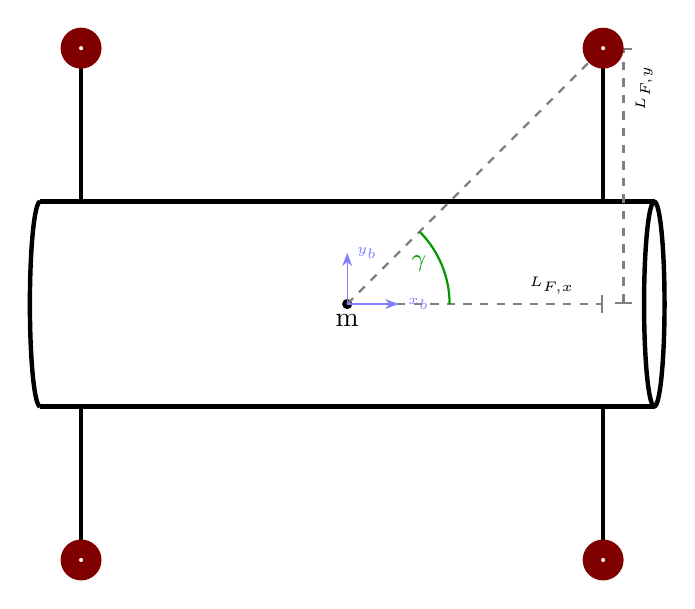
\begin{tikzpicture}[scale = 1.3]
        \draw[ultra thick] (0,1) arc (90:270:0.1cm and 1cm);
  
         \draw[ultra thick] (0,-1) -- (6,-1);
         \draw[ultra thick] (0,1) -- (6,1);
    
         \draw[ultra thick] (6,0) ellipse (0.1cm and 1cm);

         \fill[thick] (3,0) circle (0.05cm) node [below] {m};

         % Arms
         \draw[ultra thick] (0.4,1) -- (0.4,2.5);
         \draw[ultra thick] (5.5,1) -- (5.5,2.5);
         \draw[ultra thick] (0.4,-1) -- (0.4,-2.5);
         \draw[ultra thick] (5.5,-1) -- (5.5,-2.5);

         



         \draw [thick,dashed, gray][-|] (3,0) -- (5.5,0);
         \node at (5, 0) [above] {\tiny$L_{F,x}$};

 

         \draw [thick, dashed, gray] (3,0) -- (5.5,2.5);
         
         \draw [thick, dashed, gray][|-|] (5.7,0) -- (5.7,2.5);
            \node at (5.9, 1.8) [right, rotate = 90] {\tiny$L_{F,y}$};
         \draw[thick, green!60!black] (4,0) arc (0:45:1cm);

        
        \node at (3.7, 0.4) [green!60!black]{\small$\gamma$};
         % Body Frame Axis
         \draw [blue!50][-Stealth] (3,0) -- (3.5 ,0) node [right]{\tiny $x_b$};
         \draw [blue!50][-Stealth] (3,0) -- (3 ,0.5) node [right]{\tiny $y_b$};

         \fill[thick, red!50!black] (0.4,2.5) circle (0.2cm);
         \fill[thick, red!50!black] (5.5,2.5) circle (0.2cm);
         \fill[thick, red!50!black] (0.4,-2.5) circle (0.2cm);
         \fill[thick, red!50!black] (5.5,-2.5) circle (0.2cm);
         \fill[thick, white] (0.4,2.5) circle (0.02cm);
         \fill[thick, white] (5.5,2.5) circle (0.02cm);
         \fill[thick, white] (0.4,-2.5) circle (0.02cm);
         \fill[thick, white] (5.5,-2.5) circle (0.02cm);
    \end{tikzpicture}
     \caption{Geometries of H-Frame Quadrotor}
     \label{fig:Geometries}
 \end{figure}
From Figure \ref{fig:Geometries}, the motor positions are
$$\mathbf{r}_1=(L_{F,x},\,L_{F,y}),\quad \mathbf{r}_2=(-L_{F,x},\,L_{F,y}),\quad \mathbf{r}_3=(-L_{F,x},\,-L_{F,y}),\quad \mathbf{r}_4=(L_{F,x},\,-L_{F,y})$$
where $L_{F,x}=L\cos\gamma$ and $L_{F,y}=L\sin\gamma$, with $L$ the distance from the center of mass to each motor. Roll depends on the left/right thrust difference and pitch on the front/rear difference:
$$\tau_\phi = L_{F,y}K_T\left(\omega_3^2+\omega_4^2-\omega_1^2-\omega_2^2\right)$$
$$\tau_\theta = L_{F,x}K_T\left(\omega_1^2+\omega_4^2-\omega_2^2-\omega_3^2\right)$$
Therefore, the motor torque vector is
$$\boxed{\boldsymbol{\tau}_m = \begin{bmatrix}
    L_{F,y}K_T\left(\omega_3^2+\omega_4^2-\omega_1^2-\omega_2^2\right)\\[2pt]
    L_{F,x}K_T\left(\omega_1^2+\omega_4^2-\omega_2^2-\omega_3^2\right)\\[2pt]
    K_D\left(\omega_1^2-\omega_2^2+\omega_3^2-\omega_4^2\right)
\end{bmatrix}}$$
Identical motors and propellers are assumed, so a single $K_T$ and $K_D$ apply to all four.
$\tau_\psi = \sum_i s_i\left(K_D\omega_i^2 + I_m\dot\omega_i\right),\qquad s=[+1,-1,+1,-1]$



\subsection{Gyroscopic Torque}
Precession Theory shows us that:
$$\mathbf{\tau_g} = \mathbf{\omega} \times \mathbf{G_Z} \sum_{i=1}^{4} I_r \omega_i$$
Expanding this equation:
$$\mathbf{\tau_g} = \begin{bmatrix}
    \dot{\phi}\\\dot{\theta}\\\dot{\psi}
\end{bmatrix}\times \begin{bmatrix}
    0\\0\\1
\end{bmatrix} I_r (\omega_1-\omega_2+\omega_3-\omega_4)$$
$$\boxed{\mathbf{\tau_g} = \begin{bmatrix}
    \dot{\phi}\\\dot{\theta}\\\dot{\psi}
\end{bmatrix}\times\left[\begin{array}{c}
0\\
0\\
I_r \,{\left(\omega_1 -\omega_2 +\omega_3 -\omega_4 \right)}
\end{array}\right]}$$

Substituting terms back into the original equation:
$$I_b\dot{\omega} = \tau_m+\tau_g-(\omega\times I_b\omega)$$

$$\begin{bmatrix}
    I_x&0&0\\0&I_y&0\\0&0&I_z
\end{bmatrix}\begin{bmatrix}
    \ddot{\phi}\\\ddot{\theta}\\\ddot{\psi}
\end{bmatrix} = \begin{bmatrix}
    L_{F,y}K_T\,\left(\omega_3^2+\omega^2_2-\omega^2_4-\omega^2_1\right)\\
    L_{F,x}K_T\,\left(\omega_4^2+\omega^2_3-\omega^2_2-\omega^2_1\right)\\
    K_D(\omega_1^2-\omega_2^2+\omega_3^2-\omega_4^2)
\end{bmatrix}+\left( \begin{bmatrix}
    \dot{\phi}\\\dot{\theta}\\\dot{\psi}
\end{bmatrix}\times\left[\begin{array}{c}
0\\
0\\
I_r \,{\left(\omega_1 -\omega_2 +\omega_3 -\omega_4 \right)}
\end{array}\right]\right)-\left(\begin{bmatrix}
    \dot{\phi}\\\dot{\theta}\\\dot{\psi}
\end{bmatrix} \times \begin{bmatrix}
    I_x&0&0\\0&I_y&0\\0&0&I_z
\end{bmatrix}\begin{bmatrix}
    \dot{\phi}\\\dot{\theta}\\\dot{\psi}
\end{bmatrix}\right)$$
$$\begin{bmatrix}
    \ddot{\phi}\\\ddot{\theta}\\\ddot{\psi}
\end{bmatrix} = \begin{bmatrix}
    \frac{1}{I_x}&0&0\\0&\frac{1}{I_y}&0\\0&0&\frac{1}{I_z}
\end{bmatrix}\left(\begin{bmatrix}
    L_{F,y}K_T\,\left(\omega_3^2+\omega^2_2-\omega^2_4-\omega^2_1\right)\\
    L_{F,x}K_T\,\left(\omega_4^2+\omega^2_3-\omega^2_2-\omega^2_1\right)\\
    K_D(\omega_1^2-\omega_2^2+\omega_3^2-\omega_4^2)
\end{bmatrix}+\left( \begin{bmatrix}
    \dot{\phi}\\\dot{\theta}\\\dot{\psi}
\end{bmatrix}\times\left[\begin{array}{c}
0\\
0\\
I_r \,{\left(\omega_1 -\omega_2 +\omega_3 -\omega_4 \right)}
\end{array}\right]\right)-\left(\begin{bmatrix}
    \dot{\phi}\\\dot{\theta}\\\dot{\psi}
\end{bmatrix} \times \begin{bmatrix}
    I_x&0&0\\0&I_y&0\\0&0&I_z
\end{bmatrix}\begin{bmatrix}
    \dot{\phi}\\\dot{\theta}\\\dot{\psi}
\end{bmatrix}\right)\right)$$
\section{Full Equations of motions}
Our states are
\begin{itemize}
    \item X
    \item Y
    \item Z
    \item $\dot{X}$
    \item $\dot{Y}$
    \item $\dot{Z}$
    \item $\phi$
    \item $\theta$
    \item $\psi$
    \item $\dot{\phi}$
    \item $\dot{\theta}$
    \item $\dot{\psi}$
\end{itemize}

The derivatives of these states have been defined in the previous sections, and, are summarized here as the full equations of motion:\tiny
\begin{align*}
\begin{bmatrix}
    \dot{X}^G\\\dot{Y}^G\\\dot{Z}^G
\end{bmatrix} &= \underbrace{\begin{bmatrix}   c_\psi c_\theta &  c_\psi s_\theta s_\phi -  s_\psi c_\phi &  c_\psi s_\theta c_\phi +  s_\psi s_\phi \\  s_\psi c_\theta &  s_\psi s_\theta s_\phi +  c_\psi c_\phi &  s_\psi s_\theta c_\phi -  c_\psi s_\phi \\ - s_\theta &  c_\theta s_\phi &  c_\theta c_\phi  
\end{bmatrix}}_{R_b^G}\begin{bmatrix}
    \dot{x_b}\\\dot{y_b}\\\dot{z_b}
\end{bmatrix}\\\\
\begin{bmatrix}
    \ddot{X}^G\\\ddot{Y}^G\\\ddot{Z}^G
\end{bmatrix} &= \begin{bmatrix}
0\\0\\g
\end{bmatrix}-\underbrace{\begin{bmatrix}
    \frac{K_{d,x}}{m}&0&0\\0&\frac{K_{d,y}}{m}&0\\0&0&\frac{K_{d,z}}{m}
\end{bmatrix}}_{\text{Body Drag Coeff. Matrix}}
\begin{bmatrix}
    \dot{X}^G\\\dot{Y}^G\\\dot{Z}^G
\end{bmatrix} +\underbrace{\begin{bmatrix}   c_\psi c_\theta &  c_\psi s_\theta s_\phi -  s_\psi c_\phi &  c_\psi s_\theta c_\phi +  s_\psi s_\phi \\  s_\psi c_\theta &  s_\psi s_\theta s_\phi +  c_\psi c_\phi &  s_\psi s_\theta c_\phi -  c_\psi s_\phi \\ - s_\theta &  c_\theta s_\phi &  c_\theta c_\phi  
\end{bmatrix}}_{R_b^G} \underbrace{\begin{bmatrix}
    0\\0\\\frac{-1}{m}\left(K_{T_1}\omega_1^2+K_{T_2}\omega^2_2+K_{T_3}\omega^2_3 + K_{T_4}\omega_4^2\right)
\end{bmatrix}}_{\text{Motor Control Force}}\\\\
\begin{bmatrix} \dot{\phi} \\ \dot{\theta} \\ \dot{\psi} \end{bmatrix} &= \begin{bmatrix} 1 & \sin\phi\tan\theta & \cos\phi\tan\theta \\ 0 & \cos\phi & -\sin\phi \\ 0 & \frac{\sin\phi}{\cos\theta} & \frac{\cos\phi}{\cos\theta} \end{bmatrix}\begin{bmatrix} p \\ q \\ r \end{bmatrix}\\\\
\begin{bmatrix}
    \ddot{\phi}\\\ddot{\theta}\\\ddot{\psi}
\end{bmatrix} &= \underbrace{\begin{bmatrix}
    \frac{1}{I_x}&0&0\\0&\frac{1}{I_y}&0\\0&0&\frac{1}{I_z}
\end{bmatrix}}_{\text{Inverse $I_b$ Matrix}}\left( \underbrace{\begin{bmatrix}
    \dot{\phi}\\\dot{\theta}\\\dot{\psi}
\end{bmatrix}\times\left[\begin{array}{c}
0\\
0\\
I_r \,{\left(\omega_1 -\omega_2 +\omega_3 -\omega_4 \right)}
\end{array}\right]}_{\text{Gyroscopic Precession from Propellers}}-\underbrace{
\begin{bmatrix}
    \dot{\phi}\\\dot{\theta}\\\dot{\psi}
\end{bmatrix}
\times \begin{bmatrix}
    I_x&0&0\\0&I_y&0\\0&0&I_z
\end{bmatrix}\begin{bmatrix}
    \dot{\phi}\\\dot{\theta}\\\dot{\psi}
\end{bmatrix}}_{\text{Gyroscopic Cross Coupling (Eulers)}}\right)  +\underbrace{\begin{bmatrix}
    \frac{L_{F,y}}{I_x}\,\left(K_{T_1}\omega_3^2+K_{T_2}\omega^2_2-K_{T_3}\omega^2_4-K_{T_4}\omega^2_1\right)\\
    \frac{L_{F,x}}{I_y}\,\left(K_{T_1}\omega_4^2+K_{T_1}\omega^2_3-K_{T_1}\omega^2_2-K_{T_1}\omega^2_1\right)\\
    \frac{1}{I_z}(K_{D_1}\omega_1^2-K_{D_2}\omega_2^2+K_{D_3}\omega_3^2-K_{D_4}\omega_4^2)
\end{bmatrix}}_{\text{Motor Control Torques}}
\end{align*}
\begin{align*}
\begin{bmatrix}\dot X^G\\\dot Y^G\\\dot Z^G\end{bmatrix} &= \begin{bmatrix}V_X\\V_Y\\V_Z\end{bmatrix}\\[6pt]
\begin{bmatrix}\dot V_X\\\dot V_Y\\\dot V_Z\end{bmatrix} &=
\begin{bmatrix}0\\0\\g\end{bmatrix}
-\frac{T}{m}\,R_b^G\begin{bmatrix}0\\0\\1\end{bmatrix}
-\frac{1}{m}\,R_b^G\,\mathrm{diag}(K_{d,x},K_{d,y},K_{d,z})\,(R_b^G)^{\!\top}\begin{bmatrix}V_X\\V_Y\\V_Z\end{bmatrix}\\[6pt]
\begin{bmatrix}\dot\phi\\\dot\theta\\\dot\psi\end{bmatrix} &=
\begin{bmatrix}1&\sin\phi\tan\theta&\cos\phi\tan\theta\\0&\cos\phi&-\sin\phi\\0&\frac{\sin\phi}{\cos\theta}&\frac{\cos\phi}{\cos\theta}\end{bmatrix}
\begin{bmatrix}p\\q\\r\end{bmatrix}\\[6pt]
\begin{bmatrix}\dot p\\\dot q\\\dot r\end{bmatrix} &=
I_b^{-1}\left(
\underbrace{\boldsymbol\tau}_{\text{motor torques}}
-\underbrace{\boldsymbol\omega\times I_b\boldsymbol\omega}_{\text{Euler coupling}}
-\underbrace{\boldsymbol\omega\times\begin{bmatrix}0\\0\\-J_r\Omega_r\end{bmatrix}}_{\text{prop gyroscopic}}
\right),\quad \boldsymbol\omega=\begin{bmatrix}p\\q\\r\end{bmatrix}\\[6pt]
\boldsymbol\tau &=
\begin{bmatrix}
L_{F,y}\left(K_{T_2}\omega_2^2+K_{T_3}\omega_3^2-K_{T_1}\omega_1^2-K_{T_4}\omega_4^2\right)\\
L_{F,x}\left(K_{T_3}\omega_3^2+K_{T_4}\omega_4^2-K_{T_1}\omega_1^2-K_{T_2}\omega_2^2\right)\\
K_{D_1}\omega_1^2-K_{D_2}\omega_2^2+K_{D_3}\omega_3^2-K_{D_4}\omega_4^2
\end{bmatrix}
\end{align*}
\section{drawings}
\subsection{Top View}
\begin{center}
    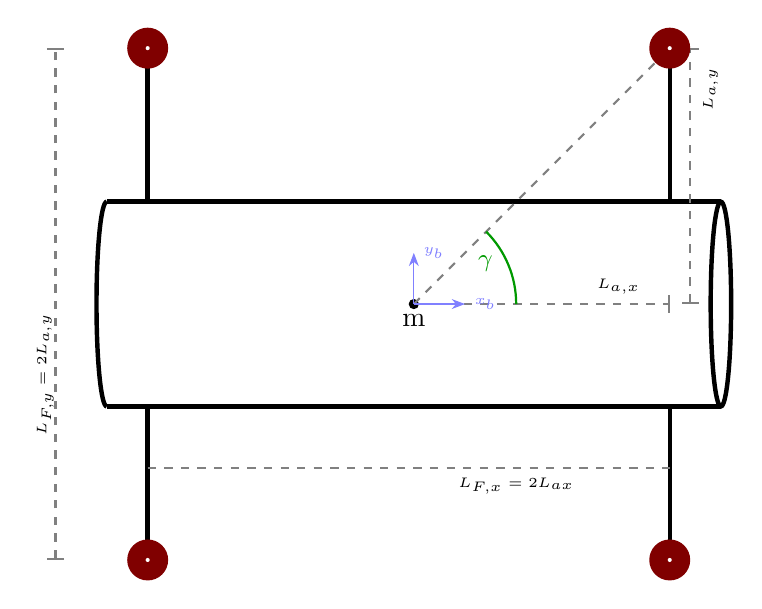
\begin{tikzpicture}[scale = 1.3]
        \draw[ultra thick] (0,1) arc (90:270:0.1cm and 1cm);
  
         \draw[ultra thick] (0,-1) -- (6,-1);
         \draw[ultra thick] (0,1) -- (6,1);
    
         \draw[ultra thick] (6,0) ellipse (0.1cm and 1cm);

         \fill[thick] (3,0) circle (0.05cm) node [below] {m};

         % Arms
         \draw[ultra thick] (0.4,1) -- (0.4,2.5);
         \draw[ultra thick] (5.5,1) -- (5.5,2.5);
         \draw[ultra thick] (0.4,-1) -- (0.4,-2.5);
         \draw[ultra thick] (5.5,-1) -- (5.5,-2.5);

         

         % Dimensions
         \draw [thick, dashed, gray] (0.4,-1.6) -- (5.5,-1.6);
         \node at (4, -1.6) [below] {\tiny$L_{F,x} = 2L_{ax}$};

         \draw [thick,dashed, gray][-|] (3,0) -- (5.5,0);
         \node at (5, 0) [above] {\tiny$L_{a,x}$};

         \draw [thick,dashed, gray][|-|] (-0.5,-2.5) -- (-0.5,2.5);
         \node at (-0.6, 0) [left, rotate = 90] {\tiny$L_{F,y}=2L_{a,y}$};

         \draw [thick, dashed, gray] (3,0) -- (5.5,2.5);
         
         \draw [thick, dashed, gray][|-|] (5.7,0) -- (5.7,2.5);
            \node at (5.9, 1.8) [right, rotate = 90] {\tiny$L_{a,y}$};
         \draw[thick, green!60!black] (4,0) arc (0:45:1cm);

        
        \node at (3.7, 0.4) [green!60!black]{\small$\gamma$};
         % Body Frame Axis
         \draw [blue!50][-Stealth] (3,0) -- (3.5 ,0) node [right]{\tiny $x_b$};
         \draw [blue!50][-Stealth] (3,0) -- (3 ,0.5) node [right]{\tiny $y_b$};

         \fill[thick, red!50!black] (0.4,2.5) circle (0.2cm);
         \fill[thick, red!50!black] (5.5,2.5) circle (0.2cm);
         \fill[thick, red!50!black] (0.4,-2.5) circle (0.2cm);
         \fill[thick, red!50!black] (5.5,-2.5) circle (0.2cm);
         \fill[thick, white] (0.4,2.5) circle (0.02cm);
         \fill[thick, white] (5.5,2.5) circle (0.02cm);
         \fill[thick, white] (0.4,-2.5) circle (0.02cm);
         \fill[thick, white] (5.5,-2.5) circle (0.02cm);
    \end{tikzpicture}
\end{center}
\section{Drawings}
\begin{center}
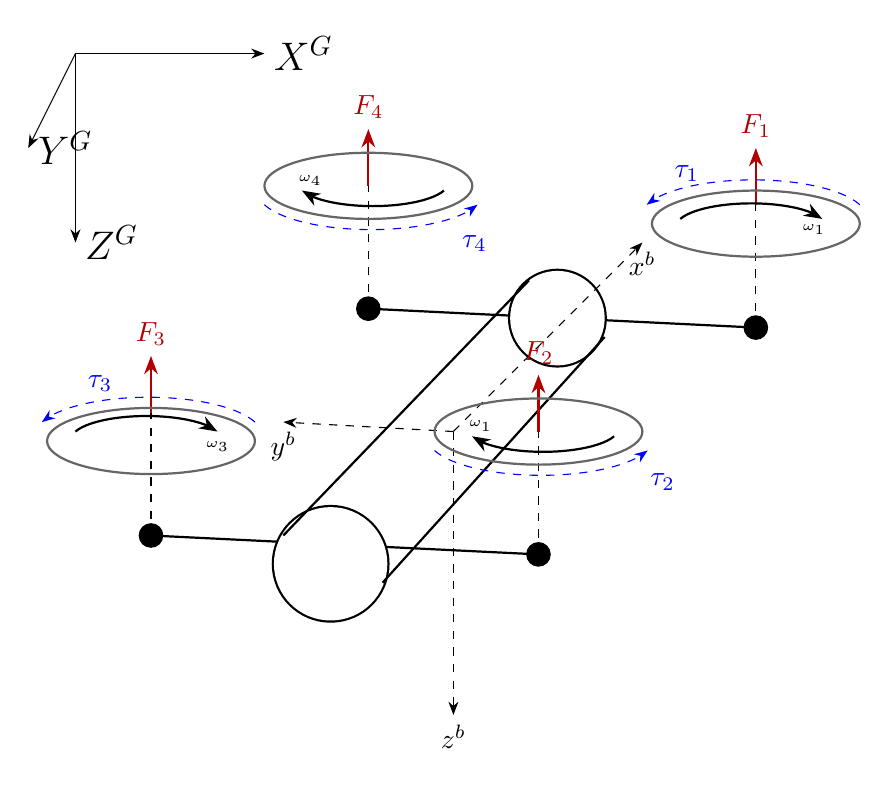
\begin{tikzpicture}[scale=1.2, >=Stealth, font=\sffamily]

  % Define key coordinates (3D projection)
  \coordinate (O) at (0, 0);          % Center origin
  \coordinate (M1) at (3.2, 1.1);     % Motor 1 (Front/Right)
  \coordinate (M2) at (0.9, -1.3);    % Motor 2 (Rear/Right)
  \coordinate (M3) at (-3.2, -1.1);   % Motor 3 (Rear/Left)
  \coordinate (M4) at (-0.9, 1.3);    % Motor 4 (Front/Left)
  

  % Draw Body Frame Axes
  % x^b axis (dashed extend past motor 1)
  \draw[thick] (M3) -- (M2);
  \draw[thick] (M1) -- (M4);
  \draw[ultra thick] (M1) ++(-4.5, -2.5) ellipse (0.6cm and 0.6cm);
  \draw[ultra thick] (M1) ++(-2.1, 0.1) ellipse (0.5cm and 0.5cm);
  \fill[white] (M1) ++(-4.5, -2.5) ellipse (0.6cm and 0.6cm);
  \fill[white] (M1) ++(-2.1, 0.1) ellipse (0.5cm and 0.5cm);
\draw [thick](-1.8,-1.1) --(0.8,1.6);
\draw [thick](-0.75,-1.6) --(1.6,1);
  % z^b axis (pointing downwards)
  \draw[dashed, ->] (O) -- (0, -3) node[below] {$z^b$};
  \draw[dashed, ->] (O) -- (2, 2) node[below] {$x^b$};
  \draw[dashed, ->] (O) -- (-1.8, 0.1) node[below] {$y^b$};

  % Motor Hubs (Filled Rounded Rectangles/Nodes)
  \foreach \m in {M1, M2, M3, M4} {
    \node[draw, fill=black, circle, inner sep=3pt] at (\m) {};
  }
    \draw [-Stealth](-4,4) -- (-2,4) node [right] {\Large $X^G$};
    \draw [-Stealth](-4,4) -- (-4,2) node [right] {\Large $Z^G$};
    \draw [-Stealth](-4,4) -- (-4.5,3) node [right] {\Large $Y^G$};
    
  % --- MOTOR 1 (Counter-Clockwise Rotation) ---
  \draw[dashed] (M1) -- ++(0, 1.3);
  \draw[thick, ->,red!70!black] (M1) ++(0, 1.3) -- ++(0, 0.6) node[above] {$F_1$};
  % Rotor Disk
  \draw[thick, gray!80!black] (M1) ++(0, 1.1) ellipse (1.1cm and 0.35cm);
  % Rotation arrow inside
  \draw[thick, ->] (M1) ++(-0.8, 1.15) arc (160:20:0.8cm and 0.25cm) node [below,pos=0.9] {\tiny $\omega_1$};
  % Torque arrow outside
  \draw[dashed, ->,blue] (M1) ++(1.1, 1.3) arc (20:160:1.2cm and 0.4cm) node[pos = 0.9, above right=2pt] {$\tau_1$};

  % --- MOTOR 2 (Clockwise Rotation) ---
  \draw[dashed] (M2) -- ++(0, 1.3);
  \draw[thick, ->,red!70!black] (M2) ++(0, 1.3) -- ++(0, 0.6) node[above] {$F_2$};
  % Rotor Disk
  \draw[thick, gray!80!black] (M2) ++(0, 1.3) ellipse (1.1cm and 0.35cm);
  % Rotation arrow inside
  \draw[thick, ->] (M2) ++(0.8, 1.25) arc (-20:-160:0.8cm and 0.25cm) node [pos=0.9, above] {\tiny $\omega_1$};
  % Torque arrow outside
  \draw[dashed, ->,blue] (M2) ++(-1.1, 1.1) arc (200:340:1.2cm and 0.4cm) node[pos = 0.9, below right=2pt] {$\tau_2$};

  % --- MOTOR 3 (Counter-Clockwise Rotation) ---
  \draw[dashed] (M3) -- ++(0, 1.3);
  \draw[thick, ->,red!70!black] (M3) ++(0, 1.3) -- ++(0, 0.6) node[above] {$F_3$};
  % Rotor Disk
  \draw[thick, gray!80!black] (M3) ++(0, 1) ellipse (1.1cm and 0.35cm);
  % Rotation arrow inside
  \draw[thick, ->] (M3) ++(-0.8, 1.1) arc (160:20:0.8cm and 0.25cm) node [pos=1, below] {\tiny$\omega_3$};
  % Torque arrow outside
  \draw[dashed, ->, blue] (M3) ++(1.1, 1.2) arc (20:160:1.2cm and 0.4cm) node[pos=0.8, above right=2pt] {$\tau_3$};

  % --- MOTOR 4 (Clockwise Rotation) ---
  \draw[dashed] (M4) -- ++(0, 1.3);
  \draw[thick, ->,red!70!black] (M4) ++(0, 1.3) -- ++(0, 0.6) node[above] {$F_4$};
  % Rotor Disk
  \draw[thick, gray!80!black] (M4) ++(0, 1.3) ellipse (1.1cm and 0.35cm);
  % Rotation arrow inside
  \draw[thick, ->] (M4) ++(0.8, 1.25) arc (-20:-160:0.8cm and 0.25cm) node [above,pos = 0.9] {\tiny$\omega_4$};
  % Torque arrow outside
  \draw[dashed, ->,blue] (M4) ++(-1.1, 1.1) arc (200:340:1.2cm and 0.4cm) node[pos=0.8, below right=2pt] {$\tau_4$};
\end{tikzpicture}
\end{center}
\subsection{Top View}


\subsection{Side View}

\subsection{Relavent Frames}
\begin{figure}[H]
    \centering
    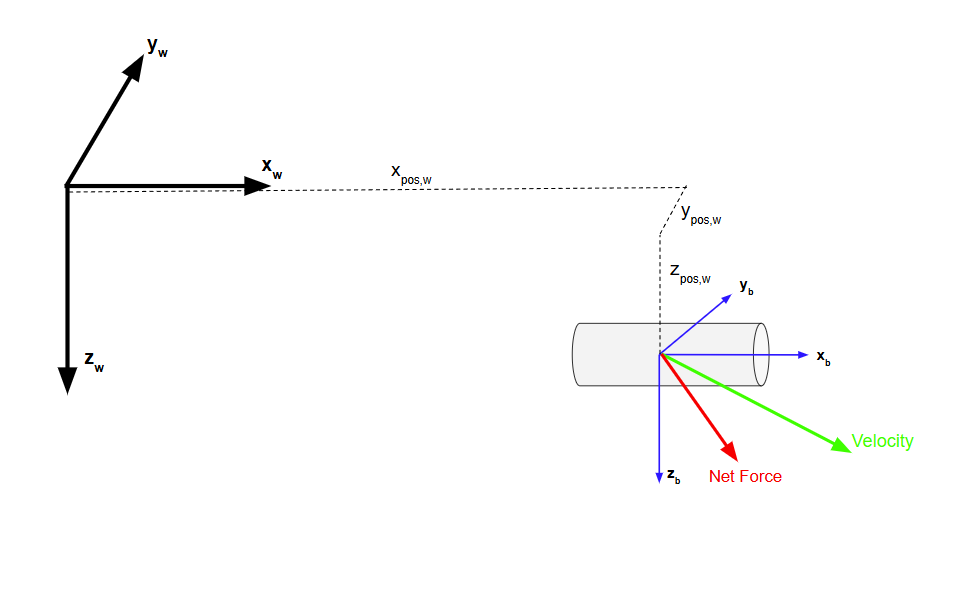
\includegraphics[width=0.5\linewidth]{fd.png}
\end{figure}

\end{document}